\chapter{Theory}
\section{Electronic Band Structure}
If the electronic configuration inside of a periodic lattice is approximated as being free, according to the stationary Schrödinger equation for electrons, an electronic dispersion relation of
\begin{equation*}
	E(k) = \frac{\hbar^2 k_n^2}{2m},
\end{equation*}
is obtained, where the possible wave vectors $k_n = n\cdot\frac{\pi}{a}$ are determined by periodic boundary conditions.
$a$ denotes the lattice parameter.
This means that the dispersion relation for free electrons inside the lattice is periodically parabolic.

The periodicity can be translated into the reduced zone scheme by mirroring.
However, at the edges of the first Brillouin zone, the electrons satisfy the Bragg condition and are therefore mirrored to the opposite side of the first Brillouin zone.
This leads to the creation of standing waves in k-space at both zone edges.
For a periodic potential generated by the nuclei in the lattice, the electron probability density is able to snap into the lowest energy solutions in two different ways:
\begin{itemize}
\item \textbf{Maxima of $|\psi|^2$ at locations of nuclei:} As a consequence of the tight Coulomb binding between the electrons and nuclei, the energy is lowered with respect to the free parabolic dispersion. The parabola is bending downwards.
	\item \textbf{Maxima of $|\psi|^2$ between locations of nuclei:} Illustratively speaking, the electrons are located further away from the nuclei. Hence, the energy is raised with respect to the free parabolic dispersion as a consequence of the looser Coulomb binding. The parabola is bending upwards.
\end{itemize}

In total, the parabola bends cause the band structure by introducing a \textit{band gap}.
Electronic states which lie inside the band gap are forbidden.
The resulting bands are now filled up, considering the Pauli exclusion principle.
At \SI{0}{\kelvin}, there are no electrons with energies above the Fermi energy $E_\text{F}$.
At room temperature, however, some electrons are thermally excited into states above the Fermi energy, since the Fermi distribution
\begin{equation*}
  \overline{n_\lambda} = \frac{1}{\e^{\beta\left(\epsilon_\lambda-\mu\right)} + 1}
\end{equation*}
is only approaching a Heaviside theta function for $T\rightarrow 0$.

Depending on the filling of these bands, a distinction is made between
\begin{itemize}
	\item \textbf{isolators:} valence band full, conduction band empty, large band gap,
	\item \textbf{semiconductors:} valence band full, conduction band empty, small band gap,
	\item \textbf{metals:} valence band full, conduction band partially full.
\end{itemize}

\section{Semiconductors}
Semiconductors are materials with a Fermi level inside their band gap at equilibrium, where the band gap is significantly smaller than that of an insulator.
Depending on the width of the band gap,
\begin{itemize}
	\item \textbf{narrow gap semiconductors}, with $0<E_\text{g}\leq\SI{0.5}{\eV}$,
	\item \textbf{ordinary semiconductors}, with $\SI{0.5}{\eV}<E_\text{g}\leq\SI{2}{\eV}$ and
	\item \textbf{wide gap semiconductors}, with $E_\text{g}\geq\SI{2}{\eV}$
\end{itemize}
are distinguished theoretically.
In practical use cases, the distinction between insulators (with $E_\text{g}\geq\SI{4}{\eV}$) is loosen up depending on the context.
For example, diamond ($E_\text{g}\approx\SI{5.5}{\eV}$) is still considered to be an ordinary semiconductor.

Two types of semiconductors may be distinguished: intrinsic semiconductors which have their Fermi level right in the middle of the band gap and extrinsic materials which are also referred to as 'doped'.

\subsection{Doping}
A pure semiconductor is not very useful, since it is neither a good insulator, nor a good conductor.
By adding impurities to or gating pure semiconductors (such as pure Si) their electrical properties may be varied in a useful manner.
Doping and gating draw either the conduction or the valence band very close to the Fermi level, greatly increasing the number of free states there.

Doping is accomplished by adding small quantities of foreign atoms to the semiconductor.
Consider for example Si from the fourth main group of the periodic system of elements which has four valence electrons that bond each silicon atom to its neighbors.
Adding either elements from the third (i.e. B, In) or fifth main group (i.e. As, P) may be used for creating p- or n-doped semiconductors, since they either lack or add one electron in their valence shells.

In \textit{p-doped} materials the so called \textit{acceptors} leave a vacant electron state (\textit{hole}) when they replace a silicon atom in the crystal.
This hole can move around the lattice and function as a charge carrier.
The acceptor levels have energies just above the valence band.
By supplying a small amount of energy, electrons from the valence band may be excited into these acceptor states and thus ionize the foreign atom, leaving a negatively charged defect behind.

Similarly, in \textit{n-doped} materials the so called \textit{donators} leave one electron free, which can contribute to the conductivity of the material.
These weakly bound electrons have energies just below the conduction band and thus can be excited very easily into conducting states by supplying a small amount of energy.

Electrons and holes are characterized by their \textit{effective masses}.
%blah blah
\section{Setup}
The experiment uses a transparent cryostat, a double-walled piece of glassware that is evacuated during the experiment, shown in \autoref{fig:cryostat}.
The probe chamber is located at the end of an elongated section of the cryostat and sits between the poles of a magnetic yoke.
The cryostat is cooled with liquid nitrogen, which is held in a toroidal storage tank.
The probe chamber is connected to the storage tank via a small tube, the flow of liquid nitrogen is limited by the static pressure due to nitrogen evaporating in the probe chamber.
Venting the probe chamber with the topmost valve regulates the pressure and in turn the flow of liquid nitrogen.

A heating coil, which is regulated by a PID controller, is used to accurately set the temperature of the probe chamber.
This gives a total temperature range of \SIrange{-180}{150}{\celsius} for the experiment.

\begin{figure}
	\centering
	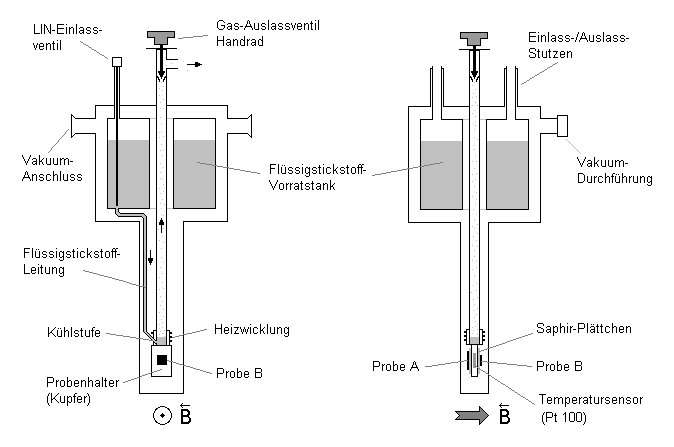
\includegraphics[width=.7\textwidth]{./img/cryostat.png}i
	\caption[Cryostat]{\textbf{The cryostat} used in the experiment}
	\label{fig:cryostat}
\end{figure}

\section{Samples}
\subsection{Sample A (Ge)}
Sample A is a block of germanium of dimensions \SI{19}{\mm} x \SI{10}{\mm} x \SI{1}{\mm}.
Contacts are made with thin gold wires, which are attached to electrolytically gold plated areas of the sample.
The exact geometry is shown in \autoref{fig:samples:ge}.

\subsection{Sample B (GaAs 2DEG)}
Sample B is a 2D electron gas inside a GaAs heterostructure.
The individual layers are depicted in the cross section \autoref{fig:samples:gaas-cross}.
The 2DEG forms between the active GaAs layer and the n-doped layer of AlGaAs.
The macroscopic shape of the sample is shown in \autoref{fig:samples:gaas-cross}.
The clover leaf or cross shaped geometry is chosen to minimize errors introduced by effects of the imperfect metal-semiconductor contact, as discussed in \autoref{sec:van-der-pauw-geometry}.

\section{Van-der-Pauw Method}\label{sec:van-der-pauw-geometry}
